
\begin{frame}

\begin{block}{Idée générale}

L'idée est de considérer les grilles de Sudoku comme les noeuds d'un graphe. On peut passer d'une grille à une autre en lui ajoutant un chiffre dans une case vide.

\bigskip

Pour appliquer A* au problème du Sudoku, on doit en modifier certains aspects :

\begin{description}
\item[Le graphe :]  le graphe doit être construit au fur et mesure que l'on développe les noeuds.

\item[L'état final :] le noeud final correspond en réalité à n'importe quelle grille complète \textit{(en ayant vérifier qu'elle ne possède pas de doublon)}

\end{description}

\end{block}
\end{frame}

\begin{frame}
\begin{block}{Construction du graphe}

On doit donc construire de nouvelles grilles quand l'algorithme doit développer un nœud. \textit{On construit autant de grille qu'il y a de valeurs possibles pour les cases vides dans la grille du noeud à développer.}

\end{block}

\begin{alertblock}{Choix des fonctions coût}

On définit bien sur des fonctions coût pour le problème :

\begin{description}
\item[G : ] on choisit le nombre de cases remplies de la grille.

\item[H : ] on prend la somme du nombre de valeurs possibles de chaque cases vides de la grille

\end{description}


\end{alertblock}

\end{frame}

\begin{frame}
\frametitle{Exemple}


\begin{minipage}{.45\textwidth}

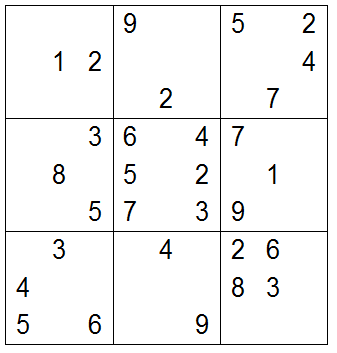
\includegraphics[scale=0.5]{images/ASTARExample/ini.png}


\end{minipage} \hfill
\begin{minipage}{.45\textwidth}

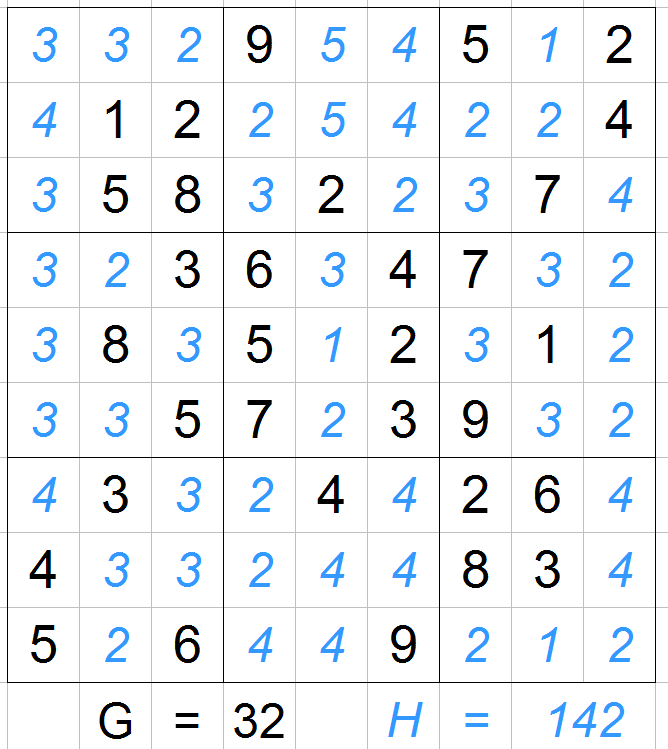
\includegraphics[scale=0.3]{images/ASTARExample/ini_H.png}

\end{minipage}

\end{frame}

\begin{frame}

\begin{minipage}{.45\textwidth}

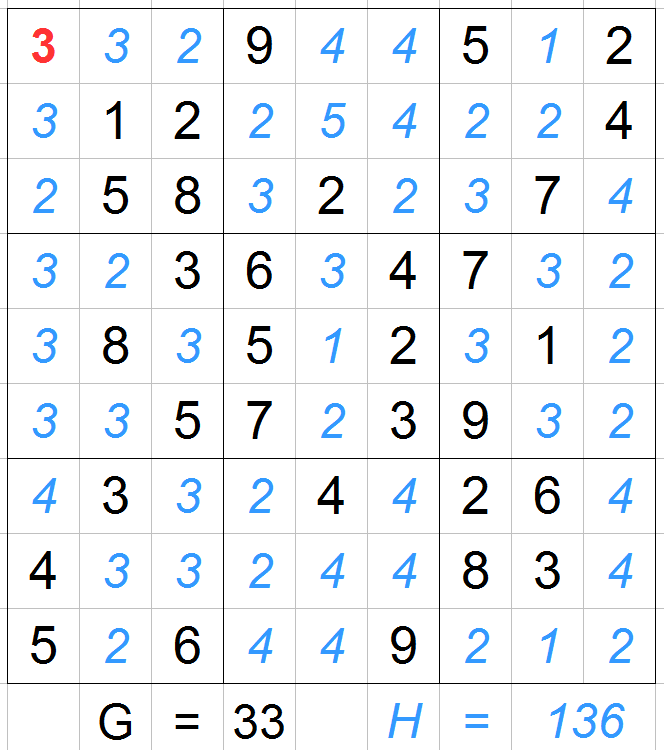
\includegraphics[scale=0.2]{images/ASTARExample/1_1.png}

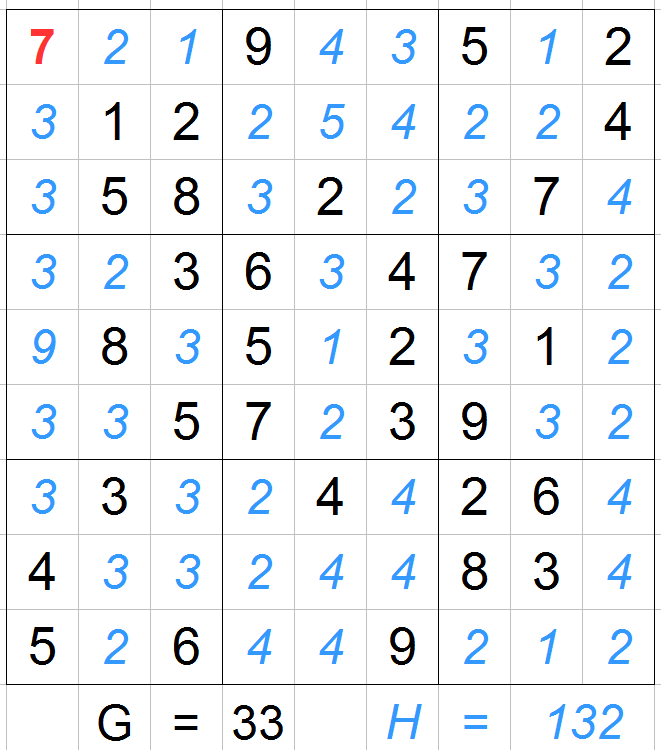
\includegraphics[scale=0.2]{images/ASTARExample/1_3.png}


\end{minipage}\hfill
\begin{minipage}{.45\textwidth}

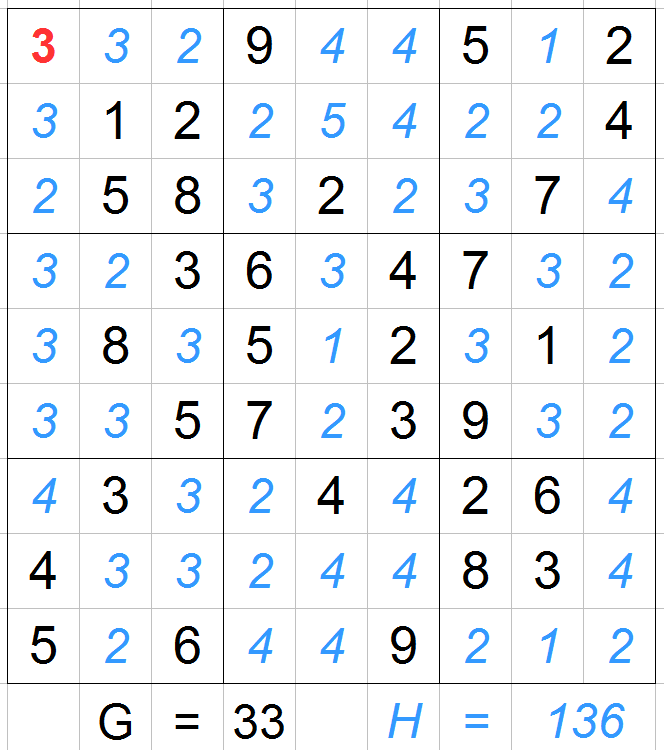
\includegraphics[scale=0.2]{images/ASTARExample/1_1.png}

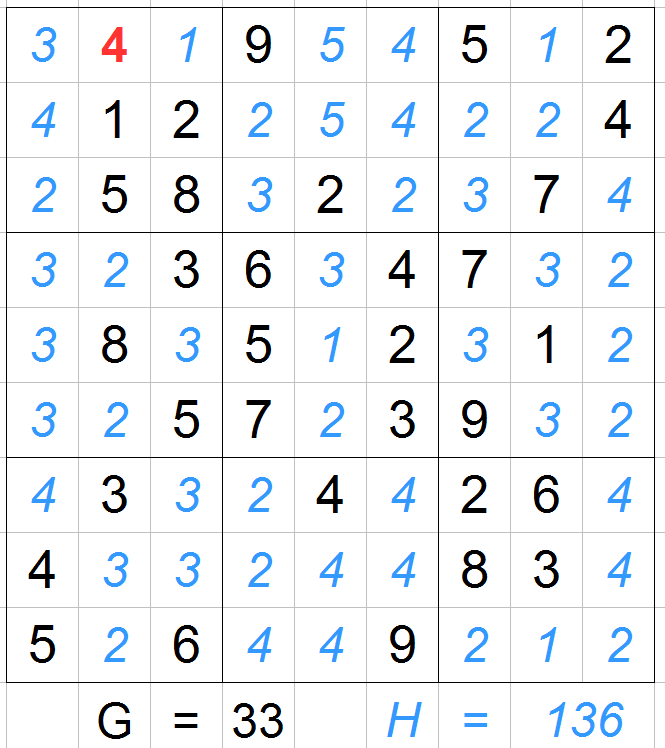
\includegraphics[scale=0.2]{images/ASTARExample/1_4.png}

\end{minipage}

\end{frame}

\begin{frame}

\begin{minipage}{.2\textwidth}
\huge{...}
\end{minipage}\hfill
\begin{minipage}{.8\textwidth}
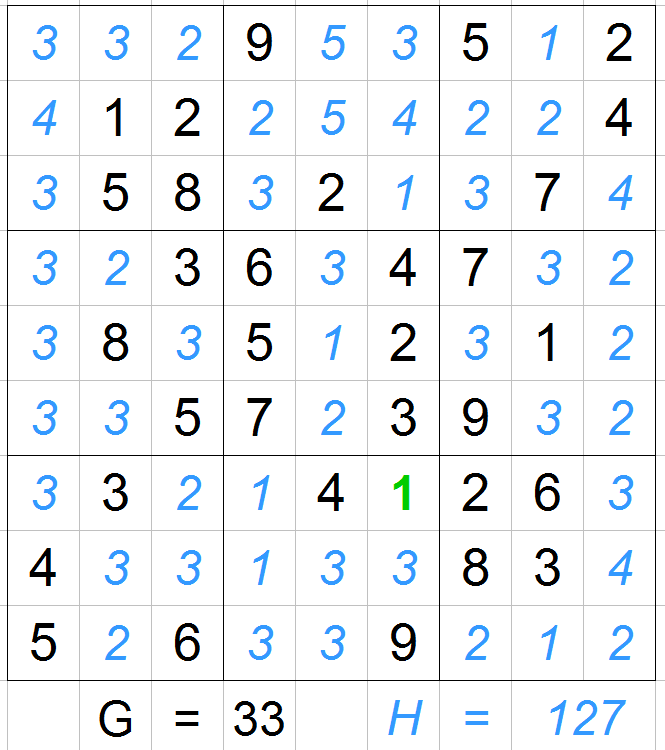
\includegraphics[scale=0.4]{images/ASTARExample/1.png}
\end{minipage}

\end{frame}

\begin{frame}

\begin{minipage}{.45\textwidth}

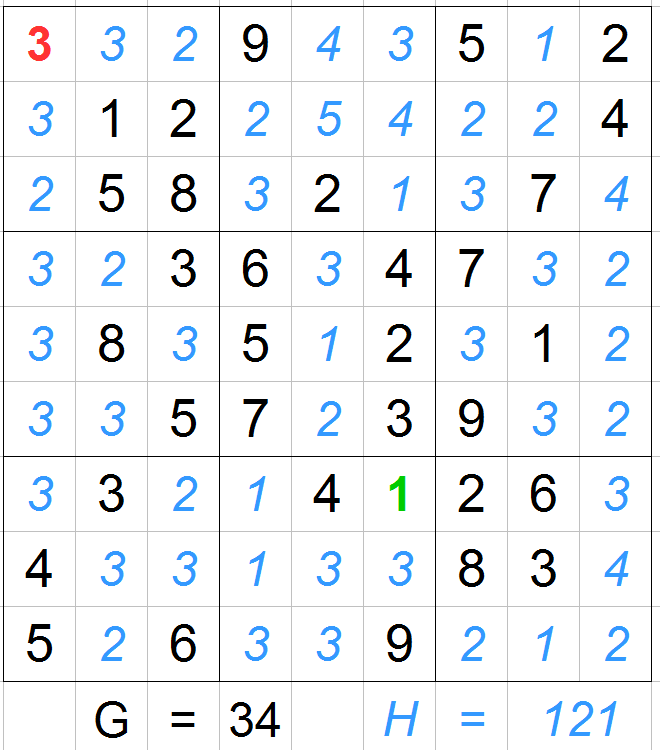
\includegraphics[scale=0.2]{images/ASTARExample/2_1.png}

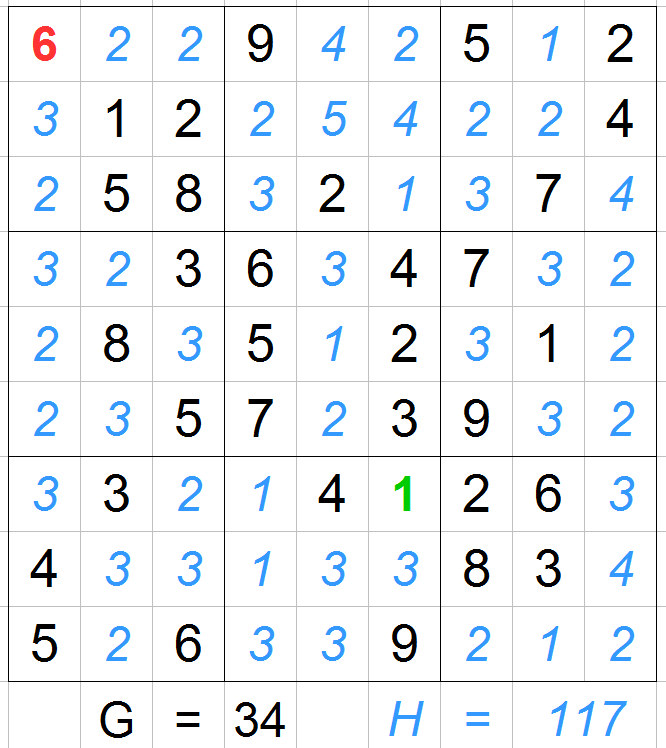
\includegraphics[scale=0.2]{images/ASTARExample/2_2.png}

\end{minipage}\hfill
\begin{minipage}{.05\textwidth}
\huge{...}

\end{minipage}\hfill
\begin{minipage}{.45\textwidth}

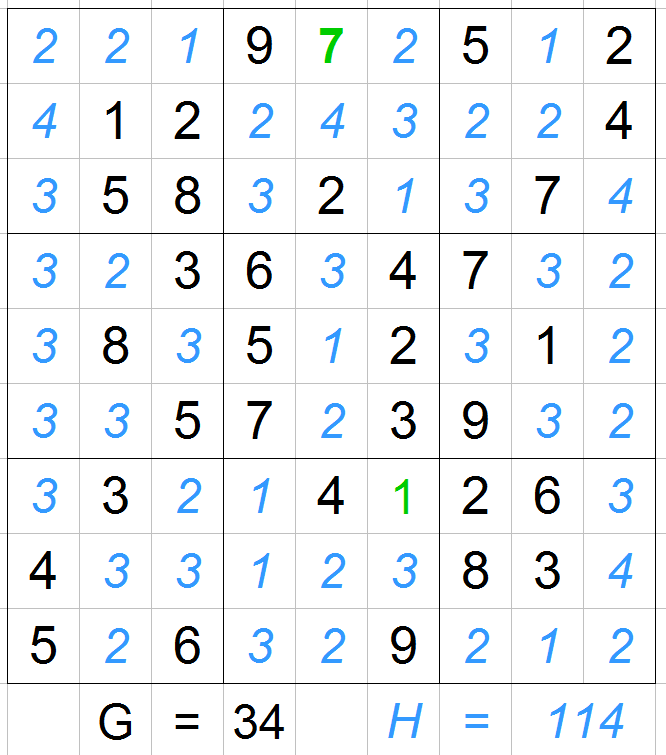
\includegraphics[scale=0.3]{images/ASTARExample/2.png}

\end{minipage}
\end{frame}

